\documentclass[a4paper]{article}
\usepackage[utf8]{inputenc}
\usepackage[danish]{babel}

\usepackage{hyperref}
\usepackage{amsmath}
\usepackage{amsfonts}
\usepackage{amssymb}
\usepackage{graphicx}
\usepackage{fancyhdr}
\usepackage{moreverb}
\usepackage{verbatim}

% Ved at bruge kommandoen \newcommand kan man forkorte kommandoer eller ændre dem til noget mere passende.
\newcommand{\setR}{\mathbb{R}}
\newcommand{\setZ}{\mathbb{Z}}
\newcommand{\setN}{\mathbb{N}}
\newcommand{\setF}{\mathbb{F}}
\newcommand{\lra}{\leftrightarrow}
\newcommand{\Lra}{\Leftrightarrow}
\newcommand{\ra}{\rightarrow}
\newcommand{\Ra}{\Rightarrow}
\newcommand{\ac}{\textasciicircum}
\newcommand{\uuline}[1]{\underline{\underline{#1}}}
\newcommand{\bpm}{\begin{pmatrix}}
\newcommand{\epm}{\end{pmatrix}}

\renewcommand{\headrulewidth}{0pt}
\title{Delrapport 4}
\author{Anders Brandhof '190493' SGL135 \\ Andreas Jørgensen '240594' SRV415 \\ Casper Iversen '090691' JVP497 \\ Søren Jensen '270792' PWS412 \\
Instruktor: Markus Lund W\\
ProjDat2015}
\begin{document}

\maketitle

\pagebreak

\tableofcontents

\newpage

\section{Abstract}
Københavns Erhvervsakademi has requested a better solution to loan computers and IT-equipment to their employees and students. Their current system is based on paper and is very time consuming. They are having trouble archiving them, and at the same time some of the papers have disappeared using this system. Our customer has therefore requested an IT-solution to store the information of the loaner computers. We are making a library lending system for their computers and IT-equipment, which will be used by their employees in their IT-department. We will create a database, which will store all the information. The information is: Their users, their computers and if a computer is available or not. Our backend will be made in Python. Our costumer has requested us to create a front-end to our liking.
\pagebreak
\section{Formål og rammer}
Formålet ved projektet er, at vi skal lave et udlåns-system for Københavns Erhvervsakademi. Dette system skal have til formål at holde opsyn med hvilke computere der er udlånt til hvilke personer og hvilke computere der er til rådighed til at blive udlånt til ansatte eller studerende i deres database.\\
Måden vi vil gøre dette på er at lave en database der skal stå for opmagasineringen af informationerne om både computerne men også hvem der har dem eller om de er klar til at blive udlånt.\\
Udover dette skal lave vi et program til at administrere data’en fra databasen og formidle den på en fornuftig måde overfor brugeren.\\
Vi skal til slut lave et program der fremviser dette på en nem forståelig måde til brugeren, så de kan indtaste hvilke computere der er udlånt til hvem og hvilke computere der er klar til udlån eller hvilke computere der bliver afleveret.\\ \\
\subsection{FACTOR Analyse}
FACTOR kan anvendes på to måder. Det kan bruges til at støtte system-definitions udviklingen, hvor det omhyggeligt overvejes, hvordan hver af de seks elementer bør formuleres. Ellers, kan der startes med en definition ved at beskrive systemet, og derefter bruge kriterene for at se, hvordan system-definitionen opfylder hver af de seks kriterier. Vi har valgt at anvende FACTOR på den først nævnte måde. \\
\textbf{Functionality:} Programmet administrerer udlån af computere i form af hvem har en computer, er en computer udlånt, og om en computer er klar til udlån samt hvor længe en person har haft en given computer.\\
\textbf{Application domain:} Anvendelsesområdet er Københavns Erhvervsakademis IT-afdeling. Dette er grundet, at det er de ansatte i afdelingen som er brugerne af systemet.\\
\textbf{Conditions:} Der er to conditions. Den ene er, at systemet skal køre på en VDI (Virtual desktop infrastructure).\\
\textbf{Technology:} Systemet vil blive kodet i Python og vil køre over python driveren ligeledes.\\
Systemet skal være tilgængeligt til at køre på  Windows, og vil komme til at have en database som vil ligge på kundens drev som bliver delt ud til kundens ansatte således at alle vil kunne bruge det derfra.\\
\textbf{Objects:} Udlåner og låner. computere og måske andre elektroniske devices.\\
\textbf{Responsibility:} Systemets ansvar ligger i, at den skal udskifte skriftlige udlånssedler, som fungerer som værdipapirer hos kunden. Dette system skal være et mere sikkert system, hvor data/sedler ikke vil kunne forsvinde, som det gør for dem nu.
\newpage
\section{Kravspecifikationer}
\subsection{Funktionelle krav}
Funktionelle krav beskriver samspillet mellem systemet og dets omgivelser uafhængigt af dens implementation. Miljøet omfatter brugeren og ethvert andet eksternt system, som systemet interagerer med. \cite[p~125]{OOSE}. De funktionelle krav beskriver altså, hvordan system skal køre. Vi har altså en liste af de ting, som er forventet systemet skal kunne. Både funktionelle og ikke-funktionelle krav har vi fundet frem via møder med kunden eller mails fra kunden.
\begin{itemize}
	\item Systemet skal kunne skanne en stregkode og modtage et brugerID som man indtaster manuelt.
	\item Systemet skal kunne modtage og opbevare en underskrift.
	\item Systemet skal kunne udskrive/sende kvittering til låneren.
	\item Systemet skal kunne udlåne og aflevere datamater.
	\item Systemet skal kunne vise data for hhv. lånerne og datamater.
	\item Systemet skal kunne have mulighed for at redigere lånerstatus og computerstatus i databasen af en bruger af systemet.
	\item Systemet skal have en hovedeside, hvor brugeren kan tilgå de forskellige funktioner.
\end{itemize}
\subsection{Ikke funktionelle krav}
Ikke-funktionelle krav beskriver aspekter af systemet, som ikke er direkte relateret til den funktionelle opførsel af systemet. Ikke-funktionelle krav omfatter en bred vifte af krav, der gælder for mange forskellige aspekter af systemet, fra usability til performance. \cite[p119]{OOSE} \\ De ikke funktionelle krav, er lidt omvendt i forhold til de hvad funktionelle krav beskriver. De ikke funktionelle krav beskriver altså ikke hvad systemet skal kunne, men hvordan det skal kunne køre. Det er altså kravne til det miljø, som systemet skal køre i.
\begin{itemize}
	\item Systemet skal kunne tilgås fra Windows 7, 8.
	\item Tilgængeligheden på programmet skal være gennem et lokalt drev.
	\item Programmet skal være sikkert, altså skal det ikke kunne hackes eller kunne tilgås udefra, altså skal man være forbundet til KEA's netværk. Det skal også være sikkert ved, at der ikke mistes data i systemet.
	\item Programmet skal køre så hurtigt som muligt, da databasen over tid kan blive meget stor.
	\item Systemet må ikke være case-sensitive. Systemet må altså ikke skelne mellem store og små bogstaver ved inputs. Dette er for at undgå brugerfejl.
\end{itemize}
\newpage
\subsection{Use-Case-model}
Use cases beskriver opførelsen af systemet, som set fra en Actor’s synspunkt. En Actor er en extern entity som interagere med systemet. En use case beskriver en funktion i systemet som en del af flere events, som giver Actor et visuelt resultat. En Actor starter en use case når de tilgår systemets funktionalitet. En use case kan starte en ny use case, og derfra hente mere information fra Actor.\cite[p~42]{OOSE} \\ \\
Vi har lavet følgende udkast, som er et udtryk for, hvordan vi forventer vores system vil køre:\\ \\
\begin{figure}[h!]
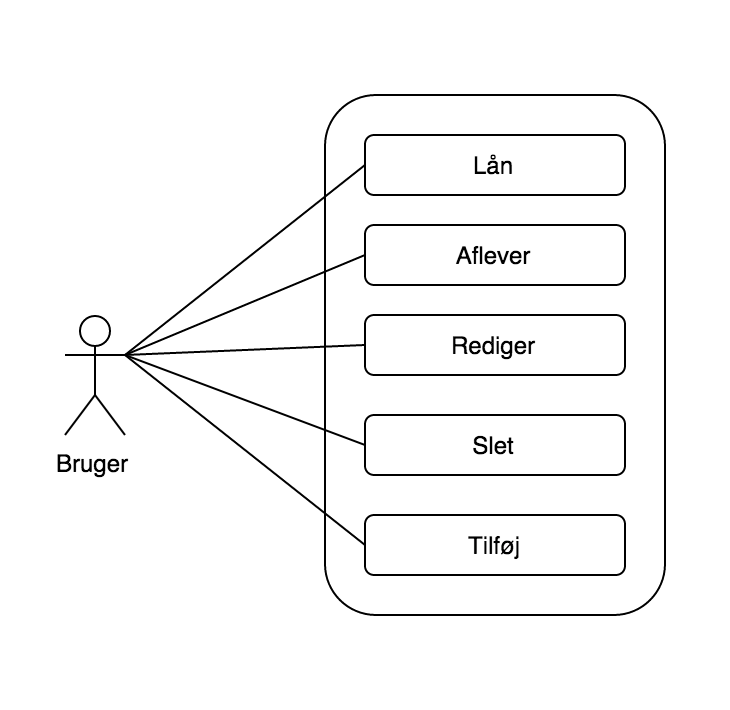
\includegraphics[width=0.8\textwidth]{UseCase}
  \caption{Use-Case-Model}
  \label{fig:USM}
  \centering
\end{figure}  \\ \\
Figur \ref{fig:USM} illusterer brugerens råderum. På figuren ses det, at brugeren skal have mulighed for at udlåne, slette, aflevere, redigere og tilføje IT-udstyr, her primært computere. Låneren har mulighed for at igangsætte et lån, eller aflevere en computer, men kun ved at henvende sig til en udlåner/bruger. Brugerne af vores system, skal have adgang til alle systemets funktioner. Der bliver derfor ikke skelnet i brugerrettigheder, da låneren kun har adgang til systemet gennem en udlåner.
\newpage
\subsection{Use-case}
Følgende use-cases er udarbejdet for at beskrive det nye, og det gamle system. Deres mening er at kaste lys over fordelene ved det nye system, såvel som bagdelene ved det gamle system. De er lavet ud fra OOSE \cite[p~44]{OOSE} og kan beskrive hvordan programmets forskellige procedurer virker, såvel som hvad der kvalificerer procedurerne, og hvornår de er udført, eller har fejlet.
\begin{table}[h]
\caption{Use-case 1}
\begin{tabular}{ll}
Use case name                 & \underline{GammeltUdlånssystem} \\ \hline
Participating actor           & \underline{Låner} \\
instances                     & \underline{Udlåner} \\ \hline
Flow of evnets                & 1. Låneren mangler en computer.\\& Låner henvender sig derfor til udlåneren for at låne en.
\\& 2. Udlåneren tjekker i arkivet, om der er en ledig \\& computer. Udlåner finder en.
\\& 3. Udlåneren giver låneren en seddel, som låneren skal udfylde: \\& Computer Mærke og model, S/N Tyveri-ID, \\& Låner, Navn, KEA login, Afdeling, Telefon/mobil, \\& Bemærkninger Underskrift, Låners underskrift \\& KEA Servicedesk Sagsnr, Udlånt af, Dato.
\\& 4. Udlåneren henter computeren til låneren og arkiverer
\\& seddelen.\\ \hline
Entry conditions & - \\ \hline
Exit conditions  & -
\end{tabular}
\end{table} \\
Det gamle udlånssytem, der vises i Use-case 1, kræver ekstra unødvendig tid fra både låner og udlåner. Udlåner riskerer også, at der går rod i papirarbejdet og at tingene forsvinder. Da systemet ikke er optimalt hverken tids eller sikkerhedsmæssigt, ønsker kunden en anden løsning på problemet. Der er ingen krav til systemet, derfor ingen entry eller exit conditions.
\begin{table}[h]
\caption{Use-case 2}
\begin{tabular}{ll}
Use case name             & \underline{NytUdlånssystem-Udlån} \\ \hline
Participating actor           & \underline{Låner} \\
instances                     & \underline{Udlåner}\\ \hline
Flow of evnets                & 1. Låner mangler en computer.	\\& Låner henvender sig derfor til udlåneren for at låne en.
\\& 2. Udlåneren tjekker i arkivet, om der er en ledig \\& computer. Låner finder en.
\\& 3. Udlåneren indtaster lånerens ID og skanner computeren.
\\& 4. Udlåneren henter computeren til låneren.\\ \hline
Entry conditions & $\bullet$ Brugeren er logget ind \\ \hline
Exit conditions  & $\bullet$ Et udlån er registreret i systemet.\\
& $\bullet$ Fejl kaldes hvis ingen ledige computere findes
\end{tabular}
\end{table}\\
Her er samme process beskrevet, blot med brug af det nye udlånssystem. Her er det tydeligt at processen er meget hurtigere og nemmere, da punkter som Mærke/model, S/N Tyveri-ID, og afdeling, etc. udfyldes automatisk. Derudover er det ikke nødvendigt at arkivere fysiske kvitteringer, der har risiko for at gå tabt.
\newpage
\begin{table}[h]
\caption{Use-case 3}
\begin{tabular}{ll}
Use case name               & \underline{NytUdlånssystem-Aflevering} \\ \hline
Participating actor           & \underline{Låner} \\
instances                     & \underline{Udlåner}\\ \hline
Flow of evnets                & 1. Låner skal aflevere en computer, som har været udlånt.
\\& Låner henvender sig derfor til udlåneren for at aflevere den.
\\& 2. Udlåneren indtaster lånerens brugerID og skanner computeren.
\\& Udlåneren arkiverer computeren. \\ \hline
Entry conditions & $\bullet$ Bruger er logget ind.\\ \hline
Exit conditions  & $\bullet$ Computeren er registreret som værende ledig\\
& $\bullet$ Fejl kaldes hvis computeren allerede var registreret som ledig
\end{tabular}
\end{table}
Til sidst er afleveringen af lånerens computer beskrevet. Som det ses er dette også hurtigt og let, da den nye afleveringsmetode, ligesom udlåningsmetoden, ikke producerer fysiske værdipapirer, der kan gå tabt. Derudover udfyldes felter som Mærke/model, S/N Tyveri-ID, og afdeling, etc. igen automatisk. \\
\begin{table}[h]
\caption{Use-case 4}
\begin{tabular}{ll}
Use case name               & \underline{VisHistorik} \\ \hline
Participating actor           & \underline{Udlåner} \\
instances\\ \hline
Flow of evnets                & 1. Udlåner skal tjekke historikken for en låner.
                            \\& 2. Udlåneren vælger visHistorik-knappen for en låner, hvilket
                            \\& får programmet til at vise lånerens historik.  \\ \hline
Entry conditions & $\bullet$ Brugeren er logget ind. \\ \hline
Exit conditions  & $\bullet$ Systemet fremviser historikken
\end{tabular}
\end{table}\\
I Use-case 4 vises hvordan proceduren for at se historikken for en computer eller en bruger foregår. Denne metode er, ligesom de andre hurtige og lette. Hvis en medarbejder ønskede at tjekke historikken via det gamle udlånssystem, fandt han/hun en stor og uoverskuelig mappe frem, hvor hvert papir repræsenterede et nyt udlån. Med denne løsning er historikken blot et tryk væk.
\newpage
\subsection{Klassediagram}
Klassediagrammer bruges til at beskrive strukturen af systemet. Klasser er abstraktioner, der angiver struktur og adfærd af et sæt objekter. Objekter er instanser af klasser, der oprettes, ændres og ødelægges under udførelsen af systemet. Klassediagrammer beskriver systemet i form af objekter, klasser, attributter, operationer, og deres sammenslutninger. \cite[p~30]{OOSE} 
\begin{figure}[h!]
\includegraphics[width=0.9\textwidth]{Klassediagram}
  \caption{Klassediagram}
    \label{fig:KLS}
  \centering
\end{figure}\\
Figur \ref{fig:KLS} viser interaktionen mellem de forskellige komponenter i systemet. Det beskrives her hvordan en udlåner låner en computer til en låner. Både lån og aflevering af en computer bliver gjort af udlåneren, og benytter sig af brugerdatabasen og computerdatabasen, og udskriver en kvittering til låneren.
\newpage
\subsection{BCE-Model}
Entity objekter repræsenterer vedvarende oplysninger der registreres af systemet. Boundary objekter repræsenterer samspillet mellem aktører og systemet. Control objekter er ansvarlig for at realisere use cases. Modellering af systemet med Entity, Boundary og Control objekter giver udviklere enkel heuristik til at skelne mellem forskellige, men beslægtede begreber.\cite[p~171]{OOSE}
\begin{itemize}
	\item Boundary
	\begin{itemize}
		\item lånComputerKnap 
		\item aflComputerKnap 
		\item tilføjBrugerKnap 
		\item tilføjComputerKnap, 
		\item visHistorikKnap 
		\item udlånsformular 
		\item afleveringsformular 
		\item visLedigeKnap 
		\item visBrugereKnap
	\end{itemize}
	\item Control
	\begin{itemize} 
		\item computerLånController 
		\item computerAflController 
		\item printerController
	\end{itemize}
	\item Entity
	\begin{itemize} 
		\item databasen 
		\item computere 
		\item logins 
		\item historik
	\end{itemize}
\end{itemize}
\newpage
\subsection{Sekvensdiagram}
Et sekvens diagram forbinder use cases med objekter. Det viser, hvordan en use case (eller scenarier) opfører sig og hvordan det fordeles blandt de deltagende objekter. Sekvens diagrammer er normalt ikke så godt et medium for kommunikation med brugeren som use cases er, da sekvens diagrammer kræver mere baggrund om notation. \cite[p~179]{OOSE} 
\begin{figure}[h!]
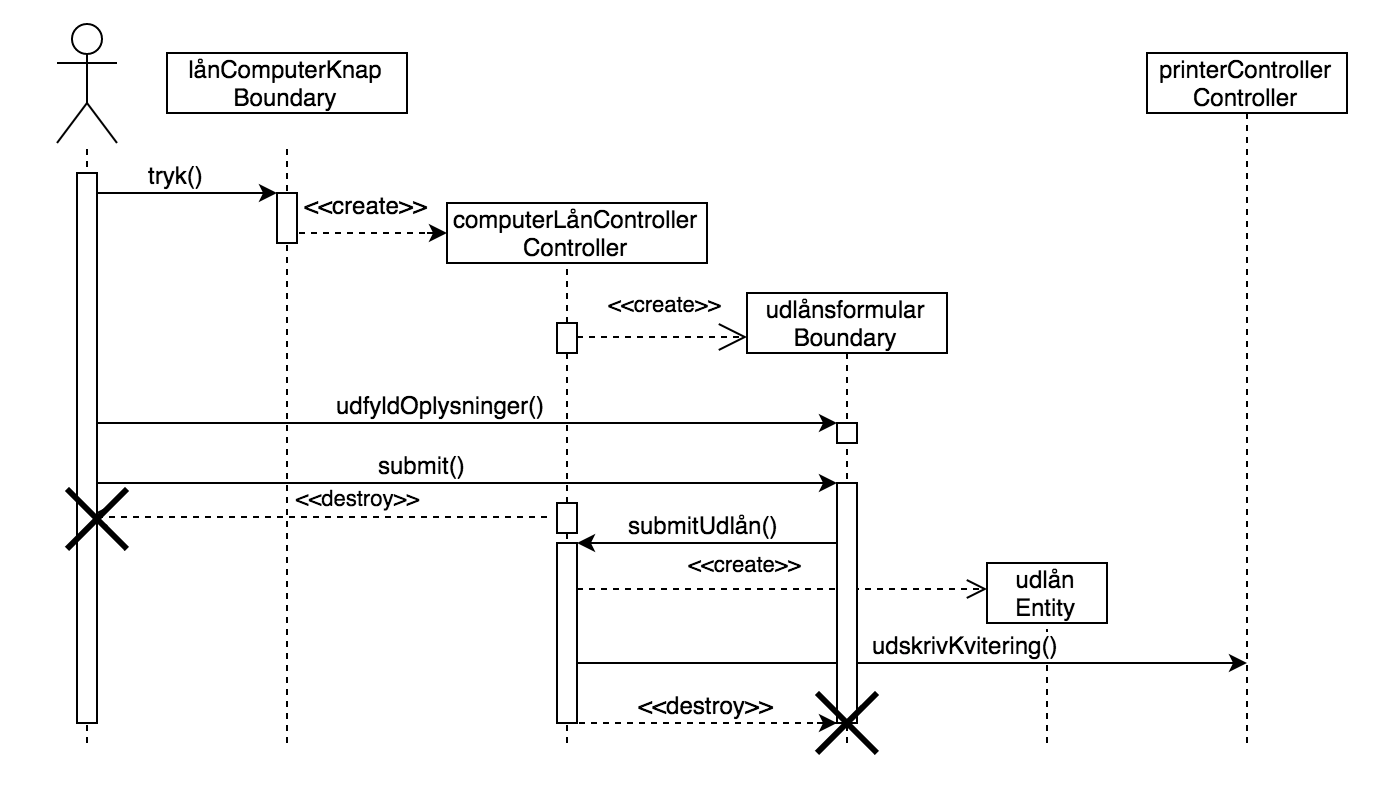
\includegraphics[width=0.9\textwidth]{SekvensLaan}
  \caption{Sekvensdiagram-1}
    \label{fig:SEK1}
  \centering
\end{figure}\\
På figur \ref{fig:SEK1} vises hvordan det nye udlånssystem kommer til at fungere ved udlån af computer. Det ses her hvordan låneren trykker på lånerknappen, hvilket skaber en controller, der skaber udlånsformularen. Denne udlånsformular udfylder og indsender låneren, hvorefter lånet oprettes i databasen, og en kvittering bliver printet.
\newpage
\begin{figure}[h!]
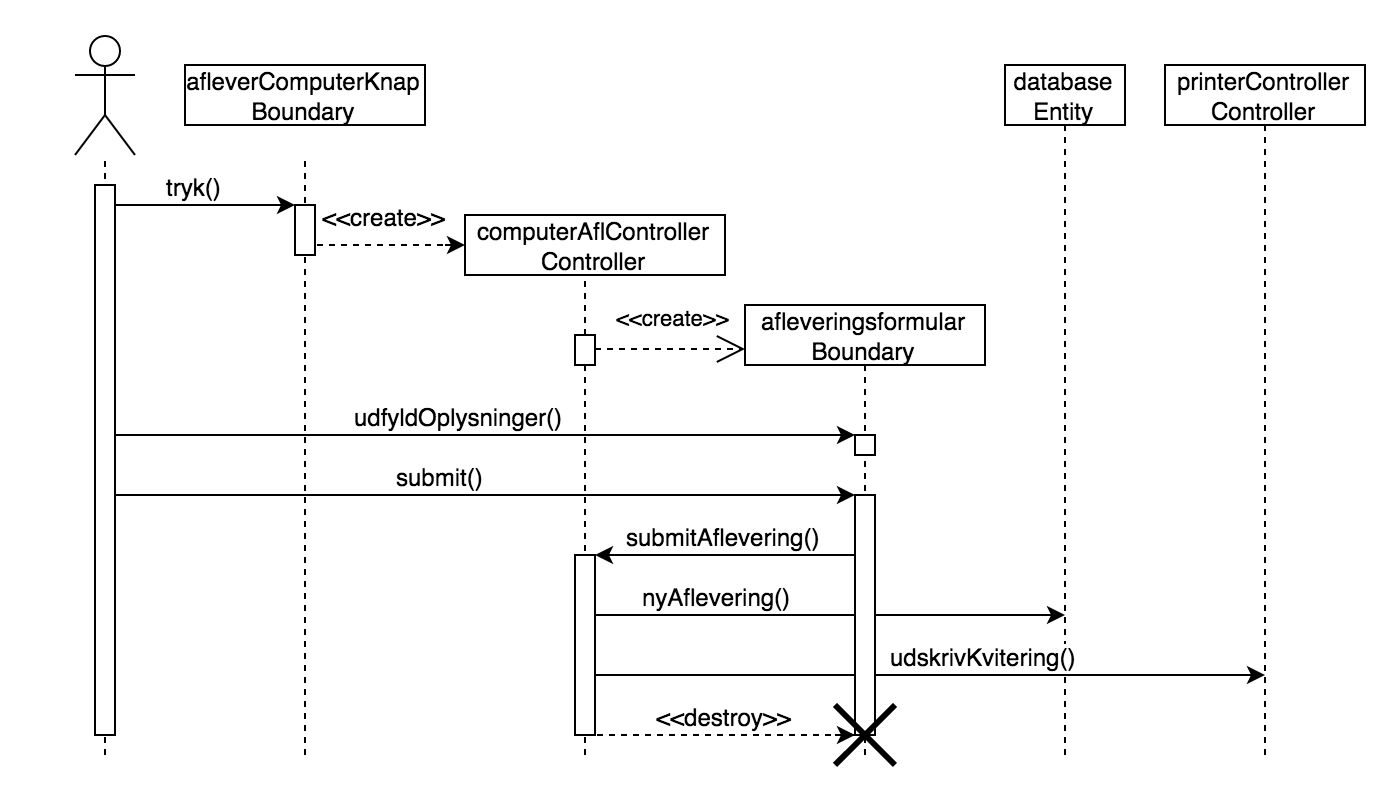
\includegraphics[width=0.9\textwidth]{SekvensAflever}
  \caption{Sekvensdiagram-2}
    \label{fig:SEK2}
  \centering
\end{figure}
På figur \ref{fig:SEK2} vises hvordan det nye udlånssystem kommer til at fungere ved aflevering af computer. Det ses her hvordan låneren trykker på afleveringsknappen, hvilket skaber en controller, der skaber afleveringsformularen. Denne afleveringsformular udfylder og indsender låneren, hvorefter computerens status ændres, så den ikke længere står som udlånt, og lånerens status ændres, så computeren ikke længere står i hans navn, og en kvittering bliver printet. Som det ses er processerne for denne og udlån af computer meget ens.
\begin{figure}[h!]
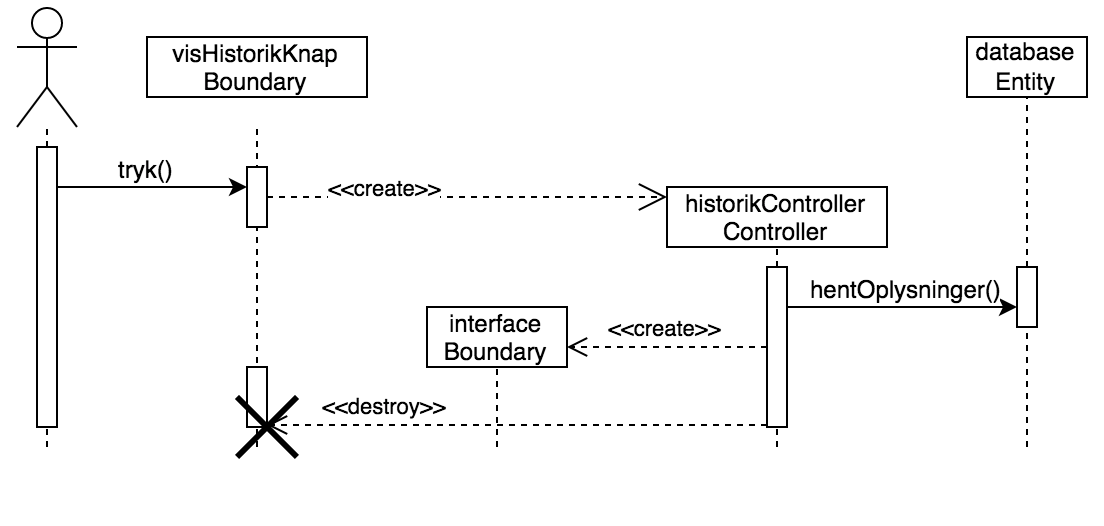
\includegraphics[width=0.9\textwidth]{SekvensHistorik}
  \caption{Sekvensdiagram-3}
    \label{fig:SEK3}
  \centering
\end{figure}\\
På figur \ref{fig:SEK3} vises det hvordan det nye udlånssystem kommer til at fungere ved vis af historik. Brugeren af programmet trykker på historikknappen for en bruger eller en computer, hvilket skaber en historikcontroller, der henter oplysninger fra databasen og skaber et interface. 
\newpage
\section{Systemdesign}
\subsection{Deployment Diagram}
% Brug NaurProgramming som reference, handler om hvordan det påvirker programmet at nye krav sættes, og derudover om man kan gå på kompromis med sit projekt så det bliver så "ændringsvenligt" så muligt
Vi har lavet et deployment diagram figur\ref{fig:DEP}, som viser vores systems implementering, det er altså hvordan og hvad der skal til for at systemet kan køre. Deployment diagrammet bliver brugt til at vise run-time komponenter og nodes. \cite[p~256]{OOSE}\\
\begin{figure}[h!]
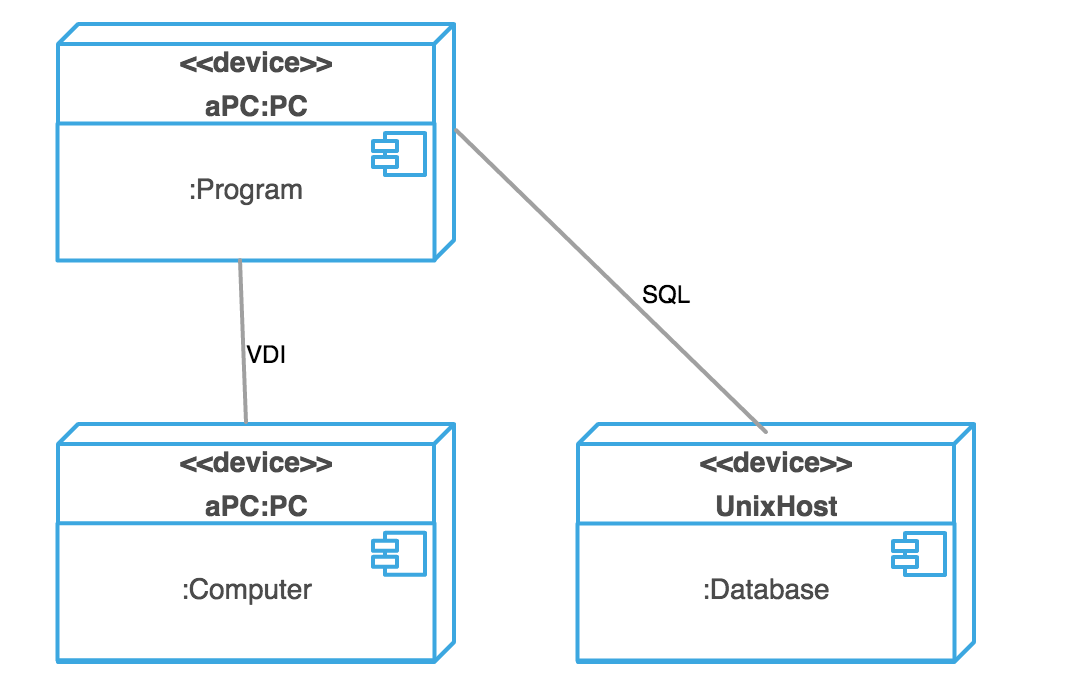
\includegraphics[width=0.9\textwidth]{deploymentdiagram}
  \caption{Deployment Diagram}
    \label{fig:DEP}
  \centering
\end{figure} \\
Figur \ref{fig:DEP} viser vores systems implementering. Vi har altså lavet en database, som taler sammen med programmet via SQL. Computeren tilgår programmet igennem en anden computer via en virtuel maskine. \\
\subsection{Database og EER-model}
\begin{figure}[h!]
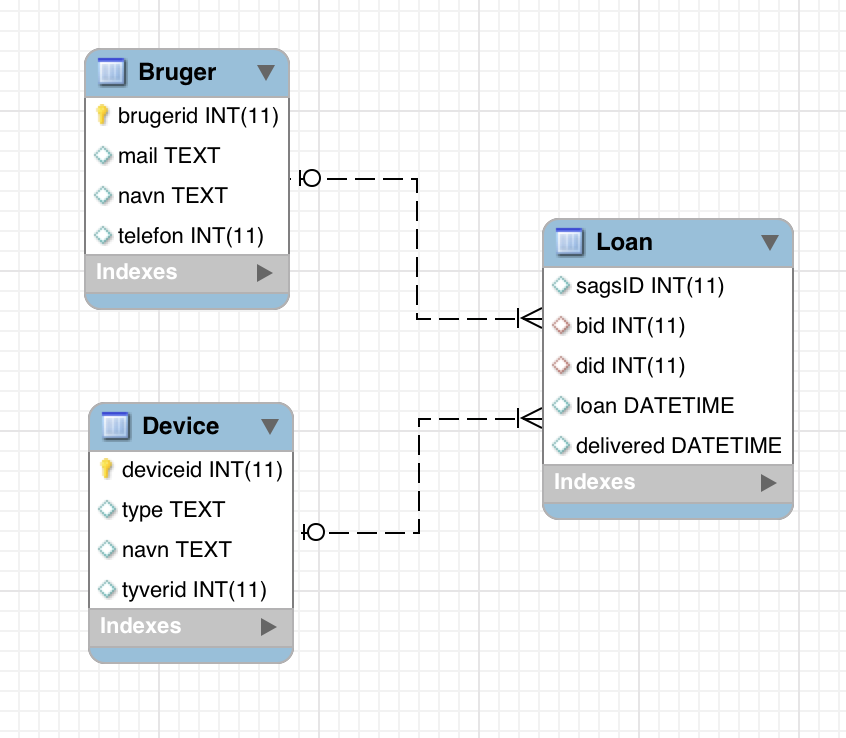
\includegraphics[width=0.8\textwidth]{EERDiagram}
  \caption{Enhanced Entity Diagram}
  \label{fig:EER}
  \centering
\end{figure}
Systemet er bygget op om en database. Databasens struktur er blevet udviklet, så det er nemt for os at udvinde den information vi eller kunden ønsker. Det er gjort, så vi med simple relationer kan få dataen frem, dette betyder, at vi ikke skal lave avanceret relationel algebra. Kravene til databasen er, at den skal opbevare data for brugerne, computerne, udlån og historikken for de udlånte computere. Vi lavede en tabel for hver af disse. Vi kom frem til den konklusion, at det ikke var nemt at udvinde information om hvilke computere var ledige, uden at man skulle slette noget af sin data i en tabellen. Dette var fordi, at når en Computer var blevet afleveret, da vil dens data stadig være i en tabel for de udlånte computere, alle afleverede computere ville altså stå som værende udlånt. Strukturen er blevet ændret til kun at indholde brugere, computere og lån, hvor historikken findes i lån. På figur \ref{fig:EER} ses et Enhanced Entity Relation diagram. Diagrammet viser databasens struktur.
\subsection{Backend/Frontend - Python Program}
Vi har i gruppen diskuteret vores forskellige muligheder for backend:
Vi har indtryk af, at Python er en af de mest brugte sprog til databaser. Vi har alle i gruppen tidligere arbejdet i Python i blok 3. Dette var i forbindelse med eksamen i Datamining. Alle i gruppen har derfor kendskab til Python.\\ \\
Vi har i gruppen også overvejet at skrive det i C++. Vi overvejede dette fordi C++ er et object-orienteret sprog, og vi alle i gruppen på forhånd har kendskab til Java. Vi har erfaret ved søgning på google, at der let kan findes information (samt dokumentation) om sproget på nettet (i forhold til f.eks. SML). Ulempen ved et valg af C++ er, at ingen i gruppen har arbejdet i C++ før, og vi vil derfor skulle lære det. \\ \\ \\
Vi er kommet frem til, at programmet vil blive skrevet i python. Vi har valgt Python, fordi vi i gruppen har de største kompetencer i dette sprog. Vi kan derfor undgå at bruge unødvendig tid på at lære et nyt sprog. \\
Vi har derfor lavet vores backend i Python, hvor vi har lavet et program, som kan hente det data vi har brug for fra databasen. Vores Python program anvender sqlite3 biblioteket. \\
Vi har ikke lavet brugerfladen endnu. Dette vil blive gjort i enten Python som et program eller blive en hjemmeside lavet i Django.\\ Grunden til hjemmesiden vil være i Django, er fordi det er et Python framework. Vi har været i kontakt med kunden omkring det skulle være et program eller en hjemmeside. Til dette havde kunden ingen krav, og lader det være op til os. Vi har i gruppen diskuteret de forskellige fordele og ulemper. En fordel ved at lave en hjemmeside i django er, at der kan laves en pænere brugerflade. Med en pænere brugerflade skal det forstås sådan, at oftest vil et program i f.eks. Python se skrabet ud og kan i visse tilfælde ligne noget fra 90'erne. De eksempler vi har set på en hjemmeside lavet i Django har oftest en pænere brugerflade end et '90'er program. \\
En af fordelene ved at lave et Python program er, at vi ikke har behov for at lære hvordan en hjemmeside i Django skal opbygges. Det er altså nemmere for os at lave et fungerende program, som vil leve op til kundens krav. \\
Vi har valgt at lave programmet i Python for at vi hurtigere har kunne få lavet en prototype.
\subsection{Udestående implementering i programmet}
<<<<<<< Updated upstream
Vores kunde har meget sent i forløbet stillet os det krav, at vi skal sikre os, at der kan indsættes en underskrift i systemet. Vi har endnu ikke bestemt os for hvordan dette skal gøres. Vi skal enten få underskriften fra en touchpad/mus på en computer, eller koble en tablet til computeren og få brugeren til at skrive sin underskrift på denne. Vi har da tænkt os at opbevare billedet med underskriften i en mappe på et fællesdrev, hvor vi tilknytte de enkelte underskrifter til de der tilhørende udlån. \\
$\bullet$ Fuld implementation af Front-end - Vi mangler at få udarbejdet nogen af de ønskede funktioner i programmet. \\
$\bullet$ Implementation af underskrift. - Vi mangler i gruppen, at diskutere hvordan vi vil udvide programmet til at tage imod en underskrift, samt hvordan denne underskrift skal opbevares i systemet.\\
$\bullet$ Program som udskriver kvittering, når en computer afleveres - Vi mangler i gruppen at diskutere, hvordan vi vil udvide programmet til enten automatisk at sende en kvittering til print, eller til at lave kvittering, som brugeren selv manuelt kan sende til print. Kunden ønsker at kvittering skal indeholde følgende: Computerens mærke, model, serie nummer, tyveri ID, lånerens initialer, lånerens underskrift, tilhørende sagsnummer, dato for udlevering og dato for indlevering.
=======
Vores kunde har derudover også stillet os det krav, at vi skal sikre os at der kan indsættes en underskrift i systemet. Vi har endnu ikke bestemt os for hvordan dette skal gøres. Vi skal enten få underskriften fra en touchpad/mus på en computer, eller koble en tablet til computeren og få brugeren til at skrive sin underskrift på denne. Vi har da tænkt os at opbevare billedet med underskriften i en mappe på et fællesdrev, hvor vi tilknytte de enkelte underskrifter til de der tilhørende udlån.
\begin{itemize}
	\item Fuld implementation af Front-end - Vi mangler at få udarbejdet nogle af de ønskede funktioner i programmet.
	\item Implementation af underskrift. - Vi mangler i gruppen, at diskutere hvordan vi vil udvide programmet til at tage imod en underskrift, samt hvordan denne underskrift skal opbevares i systemet.
	\item Program som udskriver kvittering, når en computer afleveres - Vi mangler i gruppen at diskutere, hvordan vi vil udvide programmet til enten automatisk at sende en kvittering til print, eller til at lave kvittering, som brugeren selv manuelt kan sende til print. Kunden ønsker at kvittering skal indeholde følgende: Computerens mærke, model, serie nummer, tyveri ID, lånerens initialer, lånerens underskrift, tilhørende sagsnummer, dato for udlevering og dato for indlevering.
\end{itemize}
\newpage
>>>>>>> Stashed changes
\section{Program- og systemtest}
Vi har tænkt os at dele program- og systemtest op i to. Vi vil her teste brugervenligheden og om systemet virker som det skal. Vores plan for at teste brugervenligheden er, at vi vil lave Think-Aloud test med vores kunde. Vi vil her observere, hvordan vores kunde færdes i vores system og give vores kunde flere forskellige opgaver som skal løses ved brug af vores system. Vi vil her undervejs notere de gode og dårlige ting ved systemet. Når testen med kunden er færdig, vil vi evaluere testen med kunden, og høre hvad kunden synes om systemet, eller om noget er uhensigtsmæssigt. Think Aloud testen vil blive lavet i forhold til artiklen "Thinking Aloud - User Testing by Molich" \cite{ThinkAloud}. \\[0.1in]
Denne test skal laves med kunden for, for det første at teste om løsningen er hensigtsmæssig, fra kundens synspunkt, og for det andet for at teste løsningens brugervenlighed og intuitivitet. 
Vi vil derudover teste vores system, for at se om det virker som det er tiltænkt. Vi vil altså lave testcases for vores funktioner i python. Vi vil her for eksempel teste, om det er muligt at låne den samme computer ud til to personer på samme tid, om det er muligt at udlåne en fri computer som har været udlånt, men er blevet afleveret. Vi vil altså teste alle de essentielle funktioner, som får systemet til at fungere. Vi vil her teste systemet i forhold til de metoder, som er nævnt i artiklen "Systematic Software Testing" \cite{SoftwareTest}.
\newpage
\section{Brugergrænseflade og interaktionsdesign}
\begin{figure}[h!]
\centering
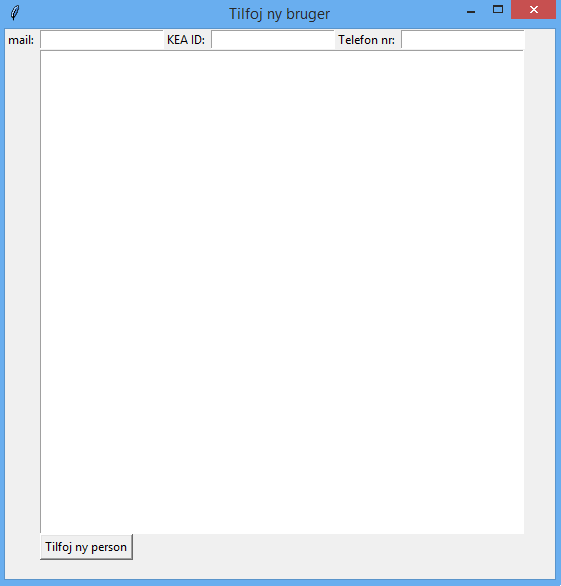
\includegraphics[width=1\textwidth]{Tilfojbruger.png}
\caption{Tilføjelse af brugere}
\label{fig:GUI1}
\end{figure}
På figur \ref{fig:GUI1} her ses vores program og hvordan bruger tilføjelsen ser ud.\\
Vi har sat det op på denne måde da for at tilføje et nyt element til databasen kræver det en mail, KEA ID (dette er det specielle id som KEA arbejdere og studerende har ligesom vi har på KU), og et telefon nummer. Vi har foruden dette også en stor text box.\\
vi har valgt at sætte det op på denne måde da det virkede som om det var den mest intuative måde at gøre det på med alle indsæt værdier i toppen og knapperne i bunden.\\
\pagebreak
\begin{figure}[h!]
\centering
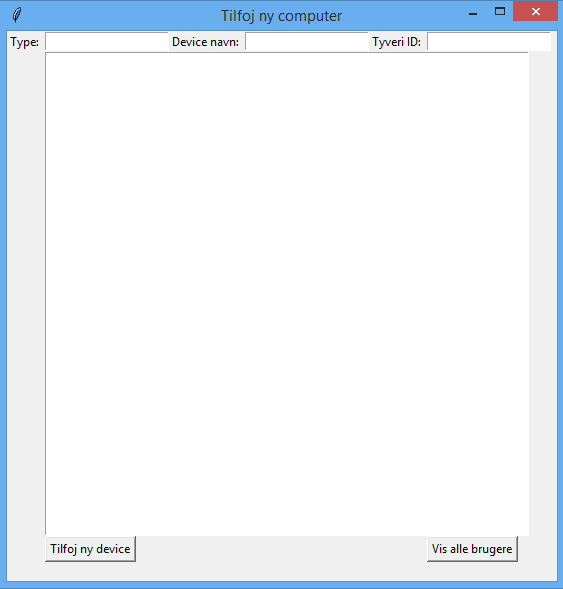
\includegraphics[width=1\textwidth]{Tilfojcomputer.png}
\caption{Tilføjelse af ny computer}
\label{fig:GUI2}
\end{figure}
\\
På figur \ref{fig:GUI2} ser vi hvordan programmet ser ud i ny computer tilføjelses delen.\\
Her har vi valgt at sætte det op på mere eller mindre samme måde som vi har gjort med tilføj bruger men bare med tilføjelse af computere og de elementer der skal til for at tilføje en ny computer til databasen.
\pagebreak
\begin{figure}[h!]
\centering
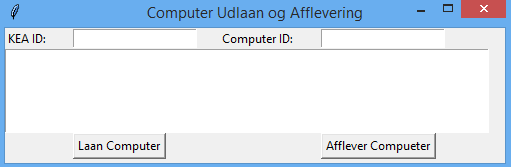
\includegraphics[width=1\textwidth]{Udlan.png}
\caption{Udlån af computere og aflevering}
\label{fig:GUI3}
\end{figure}
på figur \ref{fig:GUI3} ser vi hvordan hoveddelen af programmet ser ud, nemlig den del hvor vi realt udlåner og aflevere computere.
\pagebreak
\begin{figure}[h!]
\centering
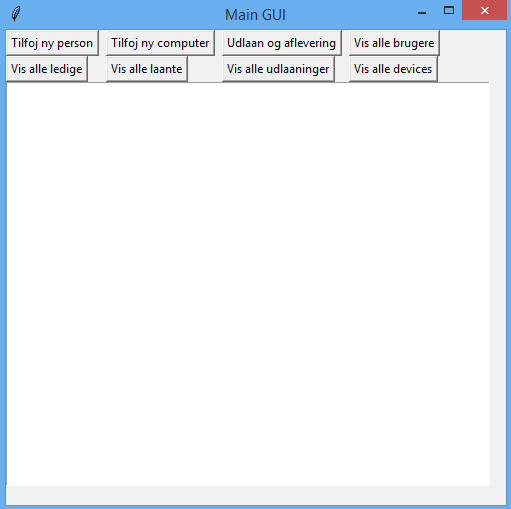
\includegraphics[width=1\textwidth]{mainGUI.png}
\caption{Udlån af computere og aflevering}
\label{fig:GUI4}
\end{figure}\\
På figur \ref{fig:GUI4} ser vi vores hoved GUI som åbner alle de andre sektioner samt mulighed for at vise alle Brugere, Devices, alle lånte devices, alle ledige devices, og alle udlåninger der nogensinde har været der.(dog kun dem som er afleveret.)
\pagebreak

\section{Projektsamarbejdet}
\subsection{Kunden}
Når vi ser på samarbejdet mellem gruppen og kunden har vi haft en del problemer i forstanden at vi ikke har haft mulighed for at få et møde i før for ret langt inde i projektet. Dette fik vi løst efter at formåede at presse på og få stablet et møde på benene. Efter det første møde 4/5 fik vi få langt støre klarhed omkring projektet. Før dette havde vi blot en email at arbejde ud fra dog gav den også godt udgangspunkt for hvad vi kunne starte med at arbejde med.\\
Vi har efter dette bedre kunne håndtere arbejdet da vi har fået langt større klarhed omkring projektet. Dog har kunden til dette mødet kommet med et meget pludseligt krav til projektet som vil tilføre en større mængde arbejde til projektet end forventet. Kravet var at vi skulle tilføje et underskrift system til, som skulle implementeres i programmet som sikkerhed for at de respektive personer havde lånt det respektive ting.\\
Vi har endnu ikke fået valgt metoden vi vil løse problemet med, men vi hælder mest til at bruge en tablet også gemme billederne lokalt eller på et virtuelt drev.\\
\subsection{Arbejdsstruktur}
For at effektivisere vores arbejde med projektet, har vi indført to faste dage hver uge, hvor vi vil sidde og udvikle IT-systemet. Dette er for at sikre, at vi kan leve op til vores egne deadlines som vi (dog kun har sat som et personligt mål da kunden ikke har en fast deadline), og nå at få den krævende viden for at få et virkende program.\\
Vi vil efter gruppearbejdet opdatere hinanden på hvad og hvor meget der er blevet lavet. Vi vil gøre det i form af forklaring af hver persons individuelle arbejde både i form af kode eller i form af hvilken strukturering af arbejdet vi hver har lavet.\\
Vi mener indtil videre ikke, at vores arbejdsindsats har været god nok, da vi har haft en del eksamener og reeksamener og derfor været nød til at udsætte arbejdet på projektet. det er derfor at vi har valgt, at ændre i vores egen møde struktur og indføre to faste dage om ugen.
Derudover har der været tryk på ifb. med nye krav for kunden som er kommet meget sent. Første møde med kunden blev stablet på benene d.4 maj, hvilket er lidt over en måned senere end hvad vi havde ønsket. Vi burde  måske have presset mere på for at få tid med kunden. Men i og med kunden er en fra gruppens chef, har vi haft problemer med at presse på da det vi var bange for at sætte vores gruppemedlem i et dårligt lys.\\
I gruppen er der omkring 3 der arbejder ad gangen, fordi der typisk er en som skal det ene eller andet, det tager vi ikke så tungt i gruppen da vi alle kan have en off-dag eller simpelthen har for travlt.\\
\subsection{Refleksion over arbejdsmetoden}
Metoden vi arbejder efter ligner meget godt Scrum metoden. ~\cite{Scrum} Vi har strukteret det således at vi mødes to gange for at evaluere vores fremgang, disse møder ligner meget disse Scrum meetings. Forskellen er at vores møder er lidt en blanding af det vi kender som "daily scrum meetings" og de reele møder. Møderne to gange om ugen sikrer en fremgang og en fælles enighed om hvordan vi går videre med projektet. Typisk bliver opgaverne delt op og derefter refkleteret til møderne. På denne måde sikrer vi os at "spilde" minimal arbejdskraft ved hele tiden at sikrer os, at det er de rigtige ting der bliver lavet og ikke eventuelt lave noget dobbelt.\\ 
\newpage
\section{Bilag 3 - Timeline}
På nuværende tidspunkt har vores arbejde ikke været på selve programmet endnu men snarere på ideen bag den, så vi vil have en bedre forståelse af hvilket produkt vi skal ende med. Dog er vores egne deadlines sat således:\\
Prototype klar den 03/05/2015 \\
Test af prototype med kunden den 04/05/2015\\
Vores timeline således ud:\\
$\bullet$ Mail modtaget fra kunde 25-03-2015:\\
Den 25. marts modtog vi mail fra kunden om hvad de ønskede sig af programmet. Kunden ønsker at få mere styr på deres proces og få elimineret deres nuværende papirseddel løsning. De ønsker, at systemet automatisk sender rykkere, men samtidig, at de også manuelt kan dette. Kunden vil gerne have, at systemet kan betjenes ved brug af en håndskanner.\\
$\bullet$ Afholdt gruppemøde 21-04-2015:\\
Den 21. april har vi aftalt, at vi ønsker at have den første prototype klar inden den 3. maj. Vi har endvidere aftalt at have to faste dage om ugen, hvor vi vil arbejde på projektet. Dette valg er truffet for at sikre os, at vores egen deadline vil kunne blive overholdt.\\
$\bullet$ Afholdt kundemøde 4-5-2015:\\
Den 4. maj holdt vi møde med kunden, hvor vi fik respons på eventuelle designs, og fik informationer om krav, prioriteringer og problemer med hensyn til løsningen. Et referat af mødet er vedlagt.
\pagebreak
\section{Referat af kundemøde d. 4. maj 2015}
\subsection*{Krav}
$\bullet$ Udlån skal indholde et underskriftsfelt \\
$\bullet$ Der skal være mulighed for udvidelse til mange computere, da systemet skal udvides i 2016. \\
$\bullet$ Computere skal have et typefelt\\
$\bullet$ Systemet må ikke kunne tilgås udefra. \\
$\bullet$ Alle skal kunne oprette nye brugere. \\
$\bullet$ Redigering er forbeholdt administratorer. \\
$\bullet$ Løsningen skal indeholde en ‘Send rykkere’-knap - Skal sende en mail fra service Desk til brugere. \\
\indent - Skal være manuel til at starte med. \\
\indent - skal kunne sendes til brugere. \\
$\bullet$ Computere skal indeholde sagsID/sagsnr. \\
$\bullet$ En kvittering skal udstedes til begge parter (KEA/låner).\\
\indent - Kan være i form af udskrift. \\
\indent - Kan være i form af mail. \\
$\bullet$ Løsningen skal indeholde et bemærkningsfelt. \\
$\bullet$ BrugerID skal være lig med KEAlogin. \\
$\bullet$ Indtastningsfelterne må ikke være case-sesitive (Store bogstaver = små bogstaver)\\
$\bullet$ Indtastningsfelterne må ikke tage højde for mellemrum.
\subsection*{Prioriterninger}
$\bullet$ Både med drop-down-menu og hyperlinks er accepteret. \\
$\bullet$ Både program og hjemmeside er accepteret så længe løsningen ikke kan tilgås udefra. \\
$\bullet$ Computerudlån er førsteprioritet - eventuelle features kan tilføjes senere. \\
$\bullet$ Manuel indtastning kan skabe menneskelige fejl, hvilket det er en acceptabel risiko indtil videre. \\
$\bullet$ Systemhastighed er en prioritet, da databasen over tid kan blive stor.
\subsection*{Problemer}
$\bullet$ Stregkoder kan være problematiske, set fra et økonomisk perspektiv. \\
$\bullet$ Python bliver muligvis et problem, da sproget skal ligge på drevet.
\newpage
\section{Reviews}
\begin{comment}
\subsection{A Rational Design Process: How and Why to Fake It}
\textbf{Hovedpunkter}\\
Den rationelle tankegang efterstræbes i artiklen, men ikke den traditionelle form af slagsen som titlen giver udtryk for.
Der henvises til en løbende udviklingsform som der ses indenfor matematikken.
F. eks. bliver et matematikbevis ikke uddybbet på den måde i starten. Det starter med en ide som der derefter arbejdes videre på løbende. Indtil der i sidste ende står et "forhåbentligvis" meget skarpere og kortere bevis end den oprindelige ide var.
Denne form for tankegang kan der draves direkte paralleller til i forhold til programmering.\\
Den rationelle metode vil aldrig kunne blive hundrede procent realiseret indenfor programmeringens verden da usikkerheder og uforudsete problemer ikke kendes på forhånd. Dertil hører mange argumenter som omhandler menneskelige fejl, mangel på specifikke/ændrende krav fra kunde, dele af ældre projekter ville måske kunne kobles på det nye osv.\\
Længere fremme i artiklen kommer det store spørgsmål på, hvorfor denne dokumentation er nødvendig før, under og efter projektet. God dokumentation for det igangværende projekt kan være altafgørende for programmøre der kommer til undervejs i et projekt og fungere som dokumentation af processen så kunde/observatører kan se fremgangen.\\\\
\textbf{Relationer og Tanker}\\
Måden som artiklen beskriver et udviklingsforløb af et projekt ligner meget Scrum metoden.~\cite{Scrum} Især i forhold til den løbende udvikling af produktet. De runs de foregår hvorved løbende prototyper/opgaver skal nåes giver god mening i forhold til denne refleksive/løbende proces af projektet.\\
Kontra bogen~\cite{OOSE} bliver der i denne artikel reflekteret meget over hvad der bliver sagt, vi vil gå så langt som at sige, at teksten er direkte kritisk overfor sig selv. Forstået i den forstand at to sider af en sag bliver taget op. Det ser man for eksempel i artiklen da den fortæller om hvorfor vi skal bruge denne rationelle desgin process, men så alligevel ikke. Bogen er meget "one-sided" i forhold til mange ting, blandt andet denne design process hvor man ikke ser denne reflektion over processen men i stedet fokuserer på at forklare de forskellige metoder.\\
\pagebreak
\subsection{Designing for Usability: Key Principles and What Designers Think}
\textbf{Hovedpunkter}\\
Artiklen sætter fokus på selve bruger-testingen. Der indikeres at for lidt energi bliver lagt i flade udtryk såsom "brugervenlighed", "nemt interface" osv. Mens det der i virkeligheden er brug for er specifik testing af de personer som skal bruge programmet, f. eks. klienten. Artiklen omtaler dette som en meget overset aspekt af udviklingen af et projekt. Der menes at man ville kunne slippe for mange "dumme fejl". Fejl som brugere vil kunne komme ud for som måske ikke så intuitive for en programmør eller designer. Man kan sige, at selve brugervenligheden kan være udsat i større projekter fordi de anses som en udgift i stedet for en nødvendighed.\\
Her starter der en sektion om hvordan man eventuelt ville kunne teste før en eneste linje kode til selve programmet overhovedet er startet.\\\\
\textbf{Relationer og Tanker}\\
Som i den anden artikel~\cite{UseDesign} er der mange antagelser og forudanselser som grundlag for mange af argumenterne. I denne kommer det for eksempel gennem generaliseringen af af hvordan diverse projekter håndteres og hvorledes deres fokuspunkter bliver prioriteret.\\
Artiklen lægger fokus på iterativt design, brugervenlighed og funktonalitet som en vigtig del af et projekts start. Dette spænder godt overens med Scrum metoden~\cite{Scrum} fordi metoden er meget iterativ igennem sine runs hvori man udbygger sit program bid for bid. Undervejs i sådan et forløb får man prototyper/versioner af sit program man kan bruge som:\\
$\bullet$Præsentation til kunder af hvor langt i projektet man er nået og hvilken funkionalitet der er nået/mangler.\\
$\bullet$Løbende versioner som kan testes på brugervenlighed og funktionalitet.\\
$\bullet$Sidst men ikke mindst sikrer man sig at have tidligere versioner af programmet man kan gå tilbage til hvis noget skulle gå galt fra version til version.
\newpage
\subsection{No Silver Bullet}
\textbf{Hovedpunkter}\\
Artiklen No Silver Bullet beskriver hvordan der ikke er nogen gylden metode med hensyn til produktivitet, pålidelighed eller enkelhed, hverken inden for systemudvikling eller ledelsesstil. Al software konstruktion indebærer væsentlige opgaver, om det er at skabe komplekse strukturer, der udgør de abstrakte softwareenheder, og utilsigtede opgaver, repræsentation af disse abstrakte enheder i programmeringssprog og kortlægning af disse på maskinens sprog inden for plads og hastighedsbegrænsninger. Mange store tidligere gennembrud indenfor softwareproduktivitet har kommet fra at fjerne de virtuelle barrierer, såsom hardwarebegrænsninger, svære programmeringssprog, og mangel på maskintid. Dette kan for eksempel gøres ved at udnytte markedet til at købe moduler, der kan købes, fremfor at konstruere det, brug af rapid prototyping, som en del af en tidlig iteration i processen. Andre metoder er at tilføje funktioner til et kørende system, som de bruges og testes, eller at finde nye gode programmører. Efterhånden som fokus på programmering øges, øges fokus på uddannelser herom også, hvilket betyder at hyring af nye hot-shot-programmører er en essentiel del af systemudvikling.\\\\
\textbf{Relationer og tanker}\\
Brooks identificerer fire essentielle problemer ved softwareudvikling: Kompleksitet, overensstemmelse, foranderlighed og usynlighed.\\
Bud på hvorfor der ikke findes en "Silver Bullet" kan være: \\
En nem løsning på noget så komplekst som systemudvikling ville være fundet for lang tid siden. Nye metoder har ofte bagsider, på punkter, der ikke med det samme anerkendes. Yderligere beklager Brooks sig om at der ikke er nok tilfældige irritationer tilbage(Mindre end $\frac{9}{10}$), til at give en betydelig systemforbedring. \\
Hvis man ser på fortiden for inden for teknologi og programmering er der kommet mange "Silver Bullets", herunder det første keyboard, den første compiler, første datanetværk, internettet, serviceorienteret arkitektur, og hundredevis af andre hjælpemidler.
\newpage
\subsection{The M.A.D. Experience}
\textbf{Hovedpunkter}\\
Denne artikel beskriver erfaringerne som er blevet opnået ved et sammensat projekt mellem en universitets forskningsgruppe og et shipping-firma, hvor der skulle udvikles en prototype for et globalt kunde service system. Forskningsgruppen havde ingen erfaringer eller tidligere viden omkring kompleksiteten ved et shipping-firma, men det lykkedes dem at levere en prototype, der langt oversteg shipping-firmaets forventninger. En af de store grunde til deres succes, var deres eksperimentale og multiperspektive tilgang til designet i praksis. Nogle af lektionerne, som blev lært for objekt-orientering er 1, Analyse er mere end at finde navneord og udsagnsord, 2 Design er mere end bare at udfylde information i en objekt-orienteret analyse model og, 3 Konsekvenser for systemudvikling i almindelighed og objekt- orientering navnlig bestå i det foreløbige respecification af den klassiske stand: analyse - design - implementering. Implikationerne for især system udvikling generelt og objekt-orientering består foreløbelig af den klassiske arbejdsmåde: Analyse, Design og Implementation\\\\
\textbf{Relationer og tanker}\\
Projektet i The M.A.D. Experience er udviklet i forbindelse med et kursus lignende PKSU, hvilket betyder at mange af metoderne, der bruges er metoder vi også bruger i dette kursus, blandt andet Mocking it up\cite{Mockup}. Derudover kræves der også en aktiv process, der foregår mellem brugeren/kundem og programmørholdet/kursisterne på samme måde som i PKSU. Dette beskrives i OOSE som Planned Communication \cite{OOSE}{p~91}. Projektet, der beskrives i artiklen er udviklet agilt med brug af Scrummetoden \cite{Scrum}. Udviklingsgruppen har på 10 uger haft 5 iterationer, og derved produceret en prototype. 
\end{comment}
\subsection{Programming as theory building}
\textbf{Hovedpunkter}\\
"Programming as theory building" handler om nogle synspunkter på programmering, der i bred forstand træffes og betragtes som en menneskelig aktivitet. Det handler om at acceptere at programmer ikke kun skal designes og produceres, men også ændres i forhold til skiftende krav. Det bliver konkluderet at det korrekte og primære mål ikke er at producere programmet, men at programmørerne bygger teorier om måden, hvorpå de aktuelle problemstillinger løses under udviklingen af programmet. Nogle af problemerne ved sådan et syn på programmering bliver diskuteret. Det er her problemer som programmets liv og modifikation, systemets udviklingsmetoder og den professionelle status af programmører, bliver diskuteret.
\newpage
\subsection{Extreme Programming}
\textbf{Hovedpunkter}\\
Extreme programming er en metode, der minder meget om den agile arbejdsmetode, inden for systemudvikling. Brugerenes krav har forsæde, og udviklerne skal altid have disse i mente i udviklingsprocessen. Undervejs i processen skal der afholdes møder mellem brugeren og udvikleren, der giver mulighed for at brugeren tilføjer nye krav, eller ændrer i gamle krav. Under disse møder skal brugeren også godkende eventuelle tilføjelser til proggrammet.\\
Extreme programming har 4 hovedprincipper:
\begin{itemize}
	\item Kommunikation: Der holdes møder mellem brugere og udviklere, omkring systemet, der er under udvikling.
	\item Simpelhed: Udviklerne skal ikke prøve at forudse problemer, men kun fokusere på de problemer, givet af brugeren.
	\item Feedback: Systemet skal løbende testes, for at give udviklerne af systemet en idé om, om hvad de laver er korrekt.
	\item Mod: Extreme programming handler om at bryde med traditionelle tankemåder. Dette kan indebære at der kræves meget grundige kravspecifikationer.
\end{itemize}
\textbf{Tanker og relationer}\\
Extreme programming minder rigtig meget om den SCRUM. På samme måde som i Extreme programming, holder vi i PSKU møder med kunden, hvor vi aftaler krav og tester, samt fremviser tilføjelser til programmet. Derudover er vi også i PKSU blevet introduceret for metoden Pair Programming, hvor to udviklere sidder sammen. Her programmerer den ene, hvor han tænker højt om alt, der vedrører programmeringen, imens den anden lytter. Denne metode drøftes der også i extreme programming, da den kan give udviklerne bedre forståelse for de problemer de støder på undervejs i processen. En anden pointe i Extreme programming er at en større udviklerstab betyder et større behov for at koordinere mellem gruppemedlemmer. Dette har ikke været et stort problem i vores udviklingsfase, da vi gennem hele processen har været 4 i gruppen. 
\newpage
\bibliography{bibte}{}
\bibliographystyle{plain}

\end{document}
